\documentclass{beamer}
\usepackage{verbatim}

\title{July 30th, 2010 - ADAM Analysis of Discrete Algebraic Models}
\author{Bonny Guang, Madison Brandon, Rustin McNeill}
\date{July 30th, 2010}

\begin{document}

%writing out applications: 
%	BMC bioinformatics site - look at papers to see what kind of examples they have.
%	-fast fixed point analysis?
%	-one would only have to see if they are biologically relevant - could get htis info really fast.	


\maketitle

\begin{frame}
	\frametitle{What we did this week}
	\begin{itemize}
	  \item{Redesigned the website}
		\item{Added code to test for positive/negative feedback circuits}
		\item{Fixed bug in Alan's code}
		\item{Complete GINsim tests and incorporated info into paper}
		\item{Figured out how to use GINsim and verified PDS output from conversion code}
		\item{Worked on paper and poster}
	\end{itemize}
\end{frame}

\begin{frame}
	\frametitle{GINsim Testing}
\begin{itemize}
	\item{27 GINsim files from the model repository tested}
	\item{Average number of nodes: 14}
	\item{Average time to compute all fixed points of a system: 0.15 seconds}
	\item{Biological system with the most nodes: 65}
	\begin{itemize}
		\item{Th cell differentiation model}
		\item{3 states (0, 1, 2)}
		\item{1.25 seconds to find the three fixed points}
	\end{itemize}
	\item{Outlier:}
	\begin{itemize}
		\item{Segment Polarity}
		\item{72 nodes, 3 states}
		\item{18 minutes to find 65 fixed points}
		\item{$2.34 \cdot 10^{34} states$}
	\end{itemize}
	\item{Longest limit cycle: one 7-cycle present}
	\item{Calculated 20 cycles for 14 systems}
\end{itemize}

	
	

\end{frame}

\begin{frame}
	\frametitle{Redesigned Website}
	\begin{figure}[h]
	\centering
	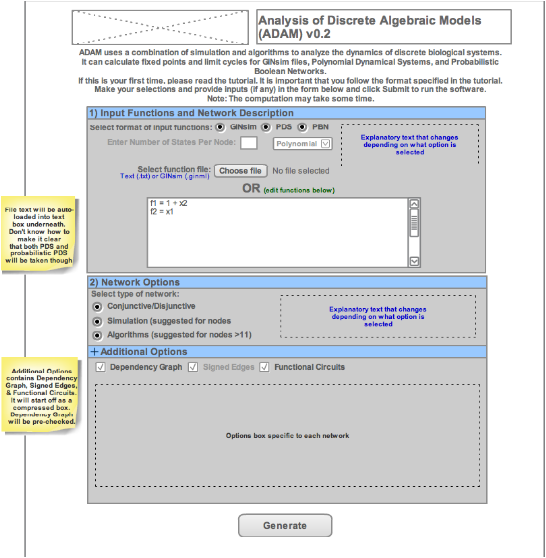
\includegraphics[scale=0.60]{websiteDesign.png}
	\caption{Screenshot of web design. Done in Gliffy}
\end{figure}
\end{frame}

\begin{frame}
	\frametitle{Plans for Next Week}
	\begin{itemize}
		\item{Polishing the paper}
		\item{Finish poster}
		\item{Decide on an application in include in Paper - look at BMC Bioinformatics site for ideas}
		\item{Implement design changes to website}
		\item{Testing of new website}
		\item{Rewrite tutorial for new website}
		\item{Make final presentation}
	\end{itemize}
\end{frame}


\end{document}
